This chapter presents the results of our research into the technical
underpinnings of the Kinect as a sensing device. Section \ref{howitworks}
describes techniques implemented in the Kinect to produces depth maps, in terms
of standard concepts from the field of machine vision. Then, section
\ref{precision} presents measurements, estimates and published data, which
together characterise the precision of the Kinect as a measurement tool.

\section{Overview: What is a Kinect}

The Kinect device is a sensor array incorporating, most notably, a system for
depth measurement. This system relies on a technique that enables low-cost
implementations. Several founders of an Israeli technology firm, PrimeSense Ltd,
invented the technique sometime before 11 October 2005 \cite{ZALEVSKY:2007}.
Microsoft corp., in turn, began selling the Kinect-branded implementation on 10
November 2010 as an optional user interface for its consumer gaming platform,
the Xbox 360.


\subsection{Specifications}

Table \ref{tab:specs} provides an overview of the electronic components that
comprise the Kinect's sensor array.

\begin{table}[ht]
\centering
\begin{tabular}{l p{10cm}}
\toprule
Component & Description \\
\midrule

RGB Camera & Sensor ``very similar'' to Mi\-cron mt9v112 (1/6" VGA CMOS) but
``larger'' and with some di\-ffering reg\-isters. Bay\-er co\-lour pa\-ttern (RG,GB).
640x\-480 pixels, 8-bit at 30 Hz.  1280x\-1024 pixels at 10\-Hz if using Open\-NI backend
, though this is referred to as ``15Hz'' in low level pro\-tocol. UYVY co\-lour
for\-mat also possible at ``15 Hz'' framerate.\cite{FREENECT}\cite{RGBDEMO} \\

Infrared camera & Monochrome CMOS sensor (no reliable source for this). Three
options for pixel size: ``small'' (unspecified); 640x480; 1280x1024. Framerate
options are 15Hz and 30Hz, except at maximum resolution (~9Hz).\cite{FREENECT}
field of view at 57 degrees horizontal, 43 degrees vertical according to retail
description.\cite{PLAY} Range reportedly ``adjustable'' (unconfirmed source) \\ 

Depth stream & Uncompressed data stream 16 bits, though this causes device
bandwidth problems. Usable options: ``differential/RLE'' compressed 11-bit
stream; 10-bit stream; 11-bit stream (uncompressed? still to be confirmed). The
only usable pixel size is 640x480. Framerate: 30Hz. \cite{FREENECT} Depth range
1.2m to 3.5m according to retail description.\cite{PLAY} Actual range
capability: ~ 0.7m-0.6m (unconfirmed source).\\

Infrared projector & Although non-reliable internet documents refe the use of a
``laser'' to project the infrared speckle pattern, this is unconfirmed. One
patent application relating to the Kinect describes a projecting a ``pattern of
coherent radiation''.\cite{SHPUNT:2010-1} Section \ref{howitworks} provides more
detail regading the projection component. \\

Accelerometer & Kionix KXSD9 Series. Sensitivity: 819 counts per g of
acceleration. Reports device tilt relative to the
horizon.\cite{FREENECT}\cite{KIONIX}\\

Microphone & ``Multiarray'' microphone consisting of four microphone units. Each
microphone generates two streams of 32 bit signed little endian PCM samples at
16KHz. A ninth channel from the device provides a unified noise-cancelled signal
in 16-bit little endian PCM samples (16KHz).\cite{FREENECT}\\

\bottomrule
\end{tabular}
\caption{Specifications of the Kinect}
\label{tab:specs}
\end{table}


\section{Theory: How it works}
\label{howitworks}

Our assessment is that the kinect measures depth using a proprietary extension
of the standard computer vision process known as stereo triangulation. In this
section we describe the depth measurement implementation in relatively high
level terms, from the perspective of theoretical computer vision. These
descriptions are based on our interpretation of public records, including
patents and scholarly as well as casual articles. We also refer, though to a
lesser extent, to our own experiments with the Kinect.


\subsection{Stereo triangulation}
\label{sub:triang}

Figure \ref{fig:triang} shows the idealised configuration of two cameras,
$c_{l}$ and $c_{r}$, set up as a stereo unit, and a point, $p$, on an object
viewed by both cameras. In this model, we simplify: 
\begin{itemize}

    \item   the sensors as pinhole cameras;

    \item   the stereo set-up so that the cameras' normal lines are parallel;

    \item   the camera planes are ``flipped'' to the front of the focal points
    for ease of illustration.

\end{itemize}

\begin{figure}[ht]
    \begin{center}
        \begin{tikzpicture}[scale=0.75,cap=round]

    % let's define some key values
    \def\xcl{-12}
    \def\xcr{-3}
    \def\yimageplanes{1.75}
    \def\imageplaneshalfwidth{1.5}
    \def\xdistoffsetf{\imageplaneshalfwidth  + 0.5}
    \def\xdistoffsetZp{\imageplaneshalfwidth  - 0.25}
    \def\ydistoffsetxl{\yimageplanes + 0.125}
    \def\ydistoffsetxr{\ydistoffsetxl}
    \def\ydistoffsetb{0}
    \def\ydistoffsetinterx{\ydistoffsetb}
    \def\xobject{-6.5}
    \def\objectdepth{9}

    % Styles
    \tikzstyle{axes}=[]

    \begin{scope}[style=axes]
    \draw[->, thick] (0,0) -- (-15,0) node (xaxis) [below] {$x$};
    \draw[->, thick] (0,0) -- (0,10) node (zaxis) [above] {$z$};
    \draw[->, very thick] (0,0) -- (0.5,-0.625) node[below] {$y$};

    \end{scope}

    % point on object
    \draw [fill, red] (-6.5,9) circle (0.05);
    \draw node [above right] at (-6.5,\objectdepth) {$p$};

    % left camera
    \draw [fill, blue] (-12,0) circle (0.05);
    \draw node [below left] at (\xcl,0) {$c_{l}$};
    % left image plane
    \draw[-, thick] (\xcl - \imageplaneshalfwidth,\yimageplanes) coordinate (ipl1)-- (\xcl + \imageplaneshalfwidth, \yimageplanes) coordinate (ipl2);

    % right camera
    \draw [fill, blue] (-3,0) circle (0.05);
    \draw node [below right] at (\xcr,0) {$c_{r}$};
    % right image plane
    \draw[-, thick] (\xcr - \imageplaneshalfwidth,\yimageplanes) coordinate (ipr1)-- (\xcr + \imageplaneshalfwidth, \yimageplanes) coordinate (ipr2);

    % depth plane
    \draw[dashed, domain=-16:3] plot (\x, {\objectdepth});

    % image rays
    \draw[dotted] (\xobject,\objectdepth) coordinate (rayl1)-- (\xcl,0) coordinate (rayl2);
    \draw[dotted] (\xobject,\objectdepth) coordinate (rayr1)-- (\xcr,0) coordinate (rayr2);

    % image points
    \coordinate (pixell) at (intersection of ipl1--ipl2 and rayl1--rayl2);
    \draw[fill, orange] (pixell) circle (0.05);
    \coordinate (pixelr) at (intersection of ipr1--ipr2 and rayr1--rayr2);
    \draw[fill, orange] (pixelr) circle (0.05);

    % focal length
    \draw[<->, thick, gray] (\xcl - \xdistoffsetf,0) -- (\xcl - \xdistoffsetf,\yimageplanes);
    \draw node [left, gray] at (\xcl - \xdistoffsetf,\yimageplanes /2) {$f$};
    
    % Camera norms
    % left
    \draw[->] (\xcl,0) coordinate (cl) -- (\xcl,\objectdepth + 1) coordinate (lnormaldepthisect);
    % perpendicular symbol
    \draw[thick] (\xcl,0.15) -| (\xcl-0.15, 0); 
    % right
    \draw[->] (\xcr,0) coordinate (cr) -- (\xcr,\objectdepth + 1) coordinate (rnormaldepthisect);
    % perpendicular symbol
    \draw[thick] (\xcr,0.15) -| (\xcr +0.15, 0); 
    %(\xcr,0)
    
    % depth
    \draw[<->, thick, gray] (\xcl - \xdistoffsetZp, 0) -- (\xcl - \xdistoffsetZp, \objectdepth);
    \draw node [below left, gray] at (\xcl - \xdistoffsetZp,{\objectdepth / 2}) {$Z_{p}$};
    
    % camera distance
    \draw[<->, very thick, gray] (\xcl,\ydistoffsetb) -- (\xcr,\ydistoffsetb);
    \draw node [below, gray] at (-7.5, \ydistoffsetb) {$b$};
    
    % left image normal offset
    \coordinate (limageplanecentre) at (intersection of ipl1--ipl2 and cl--lnormaldepthisect);
    \draw[<->, thick, gray] (limageplanecentre) -- (pixell);
    \draw node [above right, gray] at (limageplanecentre) {$x_{l}$};
    
    % right image normal offset
    \coordinate (rimageplanecentre) at (intersection of ipr1--ipr2 and cr--rnormaldepthisect);
    \draw[<->, thick, gray] (rimageplanecentre) -- (pixelr);
    \draw node [above left, gray] at (rimageplanecentre) {$x_{r}$};
    
    % inter-pixel distance
    \draw[<->, thick, gray] (pixell) -- (pixelr);
    \draw node [below, gray] at (-7.5, \ydistoffsetxr) {$b-(x_{l}+x_{r})$};

\end{tikzpicture}

        \caption{``Standard'' stereo triangulation}
        \label{fig:triang}
    \end{center}
\end{figure}

The desired value is $Z_{p}$, i.e.\ the minimum distance from the $x-y$ plane to
$p$, or the ``depth measurement'' for that point. We obtain $Z_{p}$ from: 
\begin{itemize}

    \item the focal length ($f$);

    \item the inter-camera distance ($b$); and 

    \item the respective distances between left and right camera norms and the
    pixels corresponding to $p$ on the left and right image planes ($x_{l}$ and
    $x_{r}$),

\end{itemize}

using the similarity of triangles, which yields equation
\ref{eq:triang1}.
%todo show algebra to derive this
\begin{align} \label{eq:triang1}
    \frac{Z_p}{b} = \frac{Z_p - f}{b - x_l - x_r}
\end{align}


\subsection{Stereo triangulation: the Kinect way}

Figure \ref{fig:atriang} shows the triangulation model adapted, \emph{mutatis
mutandis}, to a depth camera ($c$) projector ($s$) pair. This is sometimes
referred to as ``active triangulation'' \cite{alexander1987}, since one replaces
one passive component (a camera) with an active one (a projector). The same
simplifications apply as in section \ref{sub:triang}. The projector replaces the
second camera here, and we distinguish the target point ($p_a$) on the object
plane from the corresponding point ($p_r$) on a predetermined reference plane.

\begin{figure}[ht]
    \begin{center}
        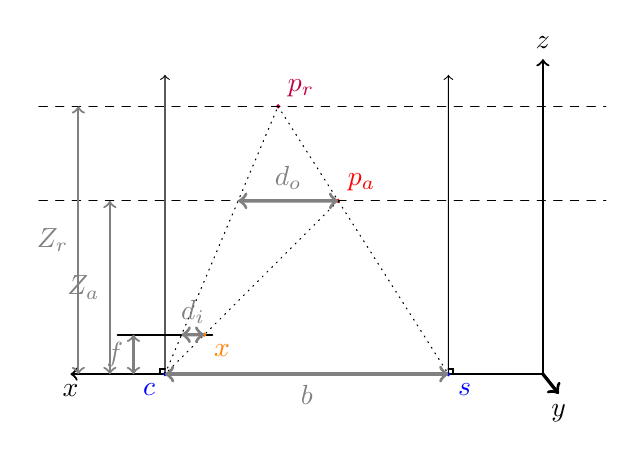
\begin{tikzpicture}[scale=0.40,cap=round]

    % let's define some key values
    \def\xc{-12}
    \def\xs{-3}
    \def\yimageplanes{1.25}
    \def\imageplaneshalfwidth{1.5}
    \def\xdistoffsetf{\imageplaneshalfwidth  + 0.5}
    \def\xdistoffsetZa{\imageplaneshalfwidth  - 0.25}
    \def\xdistoffsetZr{\imageplaneshalfwidth  - 1.25}
    \def\ydistoffsetxl{\yimageplanes + 0.125}
    \def\ydistoffsetxr{\ydistoffsetxl}
    \def\ydistoffsetb{0}
    \def\ydistoffsetinterx{\ydistoffsetb}
    \def\xobject{-6.5}
    \def\objectdepth{5.5}
    \def\referencedepth{3 + \objectdepth}
    \coordinate (pa) at (\xobject,\objectdepth);
    \coordinate (s) at (\xs,0);
    \coordinate (c) at (\xc,0);
    \coordinate (rayl2) at (\xc,0);
    \coordinate (ipll) at (\xc - \imageplaneshalfwidth, \yimageplanes);
    \coordinate (iplr) at (\xc + \imageplaneshalfwidth, \yimageplanes);


    % intersections of normals and reference plane
    \coordinate (rnrdi) at (\xs, \referencedepth);
    \coordinate (lnrdi) at (\xc, \referencedepth);
    % intersections of normals and object plane
    \coordinate (rnodi) at (\xs, \objectdepth);
    \coordinate (lnodi) at (\xc, \objectdepth);

    \coordinate (pr) at (intersection of s--pa and lnrdi--rnrdi);

    % intersection of c -- pr and object plane
    \coordinate (cprodi) at (intersection of c--pr and rnodi--lnodi);

    % pixel on image plane and expected pixel on image plane
    \coordinate (pixel) at (intersection of ipll--iplr and pa--c);
    \coordinate (epixel) at (intersection of ipll--iplr and pr--c);

    % Styles
    \tikzstyle{axes}=[]

    \begin{scope}[style=axes]
    \draw[->, thick] (0,0) -- (-15,0) node (xaxis) [below] {$x$};
    \draw[->, thick] (0,0) -- (0,10) node (zaxis) [above] {$z$};
    \draw[->, very thick] (0,0) -- (0.5,-0.625) node [below] {$y$};

    \end{scope}

    % point on object
    \draw [fill, red] (pa) circle (0.05) node [above right] {$p_a$};

    % point on reference plane
    \draw [fill, purple] (pr) circle (0.05) node [above right] {$p_r$};

    % left camera
    \draw [fill, blue] (-12,0) circle (0.05) node [below left] {$c$};
    % left image plane
    \draw[-, thick] (\xc - \imageplaneshalfwidth,\yimageplanes) -- 
        (\xc + \imageplaneshalfwidth, \yimageplanes);

    % right camera
    \draw [fill, blue] (-3,0) circle (0.05) node [below right] {$s$};

    % depth plane
    \draw[dashed, domain=-16:2] plot (\x, {\objectdepth});
     
    % Reference plane
    \draw[dashed, domain=-16:2] plot (\x, {\referencedepth});
    % p_r

    % image ray
    \draw[dotted] (pa)--(c);

    % projection ray
    \draw[dotted] (pr)--(s);
    
    % expected image ray
    \draw[dotted] (c)--(pr);

    % image points
    \draw[fill, orange] (pixel) circle (0.05) node [below right] {$x$};

    % focal length
    \draw[<->, thick, gray] (\xc - \xdistoffsetf,0) -- (\xc - \xdistoffsetf,\yimageplanes)
        node [midway, left, gray] {$f$};
    
    % Camera norms
    % left
    \draw[->] (c) -- (\xc, \referencedepth + 1);
    % perpendicular symbol
    \draw[thick] (\xc,0.15) -| (\xc-0.15, 0); 
    % right
    \draw[->] (s) -- (\xs, \referencedepth + 1);
    % perpendicular symbol
    \draw[thick] (\xs,0.15) -| (\xs +0.15, 0); 
    %(\xs,0)
    
    % actual depth
    \draw[<->, thick, gray] (\xc - \xdistoffsetZa, 0)
        -- (\xc - \xdistoffsetZa, \objectdepth)
        node [midway, left, gray] {$Z_{a}$};
    % reference depth
    \draw[<->, thick, gray] (\xc - \xdistoffsetZr, 0)
        -- (\xc - \xdistoffsetZr, \referencedepth)
        node [midway, left, gray] {$Z_{r}$};
    
    % camera distance
    \draw[<->, very thick, gray] (\xc,\ydistoffsetb) -- (\xs,\ydistoffsetb)
        node [midway, below, gray] {$b$};
    
    % point disparity over epipolar line
    \draw[<->, very thick, gray] (cprodi) -- (pa) node [midway, above, gray] {$d_o$};
    % point disparity over image plane
    \draw[<->, very thick, gray] (epixel) -- (pixel) node [midway, above, gray] {$d_i$};
    
\end{tikzpicture}

        \caption{``Active'' stereo triangulation}
        \label{fig:atriang}
    \end{center}
\end{figure}

%todo uhm, notation for lines, again?
Now it is worth emphasising the order in which the Kinect proceeds: First, for
every image pixel $x_a$ corresponding to a point ($p_a$) registered by the depth
camera, the Kinect finds the matching reference image pixel $x_r$ corresponding
to a point ($p_r$) on the reference plane by solving the so-called
``correspondence problem'' discussed in section \ref{sub:corr}. Once a matching
reference point $p_r$ is found, the Kinect determines the disparity $d_i$ along
the $x$-axis in image space between the actual image of $p_a$ and the reference
image of $p_r$. With that obtained, is it possible to derive the desired ``depth
measurement'' for the given point, or the minimum distance from the depth
camera's focal point to the object plane, from: 
\begin{itemize}

    \item the focal length ($f$);

    \item the inter-camera distance ($b$);

    \item the disparity between $x_a$ and $x_r$ along the x-axis ($d_i$);

    \item the reference image depth ($Z_r$),

\end{itemize}

using the similarity of triangles, which yields equations \ref{eq:atriang1} and
\ref{eq:atriang2}. Substituting for the common variable $d_o$, we simplify to
obtain equation \ref{eq:atriang2}.
%todo show algebra to derive this
\begin{align} 
    \frac{d_o}{b} = \frac{Z_r - Z_a}{Z_r} \label{eq:atriang1}\\
    \frac{d_i}{f} = \frac{d_o}{Z_a} \label{eq:atriang2}
\end{align}
\begin{equation} \label{eq:atriang2}
    Z_a = \frac{Z_r}{d_i \frac{Z_r}{b f} + 1}
\end{equation}

\subsection{Correspondence problem}
\label{sub:corr}

In order to ca

%todo describe experiment with pictures... 

%\subsubsection{Experiment: pattern variation over distance}

%todo describe experiment with pictures... (first discuss whether useful with Jeroen)



\section{Precision of the intrument}
\label{precision}

%todo: just take data from article
In this section we describe the Kinect's characteristics as a depth measurement
tool, and notably the precision of the measurements.


\subsection{Depth precision}

\subsubsection{Sources of error}

\subsection{Depth image resolution}

\subsubsection{Sources of error}
